\documentclass{article}
\usepackage{amssymb,amsmath,titling}
\usepackage{amssymb,mathtools,amsthm,amsmath}
\usepackage{float}
\usepackage{indentfirst}
\usepackage{listings}
\usepackage{xcolor}
%\usepackage[backend=biber]{biblatex}
%\addbibresource{refs.bib}

\definecolor{codegreen}{rgb}{0,0.6,0}
\definecolor{codegray}{rgb}{0.5,0.5,0.5}
\definecolor{codepurple}{rgb}{0.58,0,0.82}
\definecolor{backcolour}{rgb}{0.95,0.95,0.92}

\lstdefinestyle{mystyle}{
    backgroundcolor=\color{backcolour},   
    commentstyle=\color{codegreen},
    keywordstyle=\color{magenta},
    numberstyle=\tiny\color{codegray},
    stringstyle=\color{codepurple},
    basicstyle=\ttfamily\footnotesize,
    breakatwhitespace=false,         
    breaklines=true,                 
    captionpos=b,                    
    keepspaces=true,                 
    numbers=left,                    
    numbersep=5pt,                  
    showspaces=false,                
    showstringspaces=false,
    showtabs=false,                  
    tabsize=2
}

\lstset{style=mystyle}
\title{ECS 171 Final Project Report}
\author{
  Sergio Santoyo\\
  \and
  Yuan Chang\\
  \and
  Cesar Guzman Avina\\
  \and
  Will Colbert\\
  \and
  Nathaniel Faxon\\
  \and
  Kanchan Kaur\\
  \and
  Parminder Singh\\
}
\date{May 2022}

\begin{document}

\maketitle
\section{Introduction \& Background}
The stock market has evolved into a major component of our lives, as well as a reflection of the national and global economy. A stock represents ownership, or equity stake, in the company, and has served as a way for companies to raise capital. Additionally, the stock market enables individuals to grow their wealth, while holding companies accountable and keeping an eye on corporate regulation. The stock market impacts the overall economy, and therefore, impacts everyone, including non-investors. Because stock markets span all industries and sectors, it is a key factor in determining the state and cycle of the economy.

When the stock market crashes, there is a sudden decline of stock prices, which results in a loss of wealth, and are further driven by other economic factors and current events. A crash is propelled with investors selling in panic, dropping prices even more. This provides an opportunity for investors, as they can potentially buy stocks back at a much lower price.

Machine learning can be used to identify stock market and financial trends, typically done using the LSTM (Long Short-term Memory) model, support vector machines (SVM), artificial neural networks (ANN), and back propagation neural networks (BPNN). While machine learning can be used to predict stock prices and market crashes, this is a challenging problem. The stock market can be volatile, influenced by many factors, ranging from politics, unexpected events, psychological factors, a company’s performance, and so on. This dynamic nature of the stock market makes it difficult to accurately predict crashes and prices.

If a market prediction model is built to successfully predict a stock market crash, it can be beneficial to investors, while also giving a warning to companies and the general public. It can also be used in various fields/sectors. Here are a some examples: 

\newpage
	\begin{itemize}
		\item Communication and Media
			\begin{itemize}
				\item Machine learning can process content on social media platforms from high-power individuals in the stock market, and predict the market in multiple scenarios.   
			\end{itemize}
		\item Finance
			\begin{itemize}
				\item The finance sector is one of the most hit sectors during a crash. Predicting a crash could allow financial institutions to prepare for the consequences, like anticipating layoffs.
			\end{itemize}
		\item Leisure and Hospitality 
			\begin{itemize}
				\item Leisure and hospitality companies face significant economic struggles after a crash, making it difficult for smaller companies to remain in business. Predicting a crash would allow these companies to prepare for such financial hardship, while also taking some action to keep customers, like offering discounted services that can be bought ahead of time, so customers will still participate after the crash. 
			\end{itemize}
	\end{itemize}
 
\section{Literature Review} 
Machine learning techniques have several applications to the problem of market prediction. This section includes examples and methods of related work done by researchers and analysts that have developed tools and techniques that predict stock market prices and assist in proper decision making.

Zhao et al. investigated the problem of financial time series prediction by utilizing Long Short-Term Memory (LSTM) neural network as a good predictor of static and dynamic prediction. Stock data are categorized as time-series multidimensional vectors. In many cases, the time-series problem can be tackled by the LSTM. Kai Chen al. presented that a LSTM based approach used for predicting stock movements would return a $13\%$ better yield in accuracy compared to others.\cite{LSTM} Additionally more similar to the work presented in this paper is the work done by Luca Di al. indicated that using LSTM and dropout over a 5-day prediction interval with only price series data produced a $72\%$ accuracy.\cite{Time-Weighted LSTM} To test the effectiveness of a time-weighted LSTM model, Zhao et al. conduct further studies on stock indexes such as the S\&P 500 and Dow Jones Industrial Index. It concluded that when altering the model to have the best parameters, the S\&P 500 returns $80.24\%$ accuracy while a single index such as Dow Jones Industrial Index returns an $83.21\%$.\cite{RNN} The accuracy of the models in these works, though not the highest result, can still be an effective indicator in predicting the market.

\section{Dataset Description and Exploratory Data Analysis} 
The dataset used throughout this project was supplied from Kaggle. It provided us with 15032 rows which included the columns: closing, opening, low, and high prices as well as the volume, P/E ratio, \% gain and loss, and price variation for S\&P 500. Data was taken from 1962 to 2021. 
Below is a description of each column:

The following are descriptions of the features for each observation in the data-set.

	\begin{itemize}
		\item Date - Trading date (YYYY-MM-DD)
		\item Open (\#) - Market opening price
		\item High (\#) - Highest price during the trading day.
		\item Low (\#) - Lowest price during the
		\item Close (\#) - Price when the market closed for the day.
		\item Adjusted Close (\#) - Closing price after corporate actions are accounted for.
		\item Volume (\#) - Number of shares traded during the trading day.
%		\item \% Gain/Loss (\#) - Percentage Change between 2 consecutive closing prices. (Shows the gain/loss between 2 trading days)
%		\item Price Variation (\#) - Price fluctuation during the day. ((high-low)/Close)
	\end{itemize}
	
The dataset was selected because of the extensive range of dates it includes as well as the amount of details it has for each date. Overall there is a general trend upwards in the data relating to the Open, Close, High, Low, and Volume. As seen in the plots below:
\begin{center}
	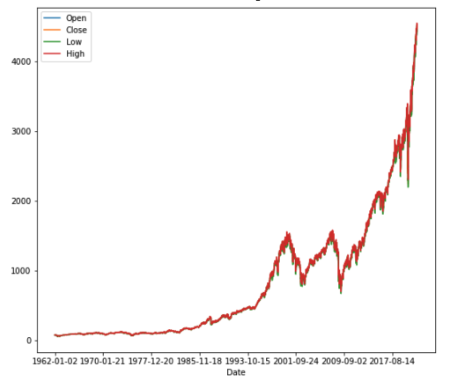
\includegraphics[scale=0.4]{p1.png}
\end{center}
\section{Proposed Methodology} 
\section{Experimental Results} 
\section{Conclusion and Evaluation} 

\begin{thebibliography}{9}
\bibitem{LSTM}
K. Chen, Y. Zhou and F. Dai, "A LSTM-based method for stock returns prediction: A case study of China stock market," 2015 IEEE International Conference on Big Data (Big Data), 2015, pp. 2823-2824, doi: 10.1109/BigData.2015.7364089.

\bibitem{Time-Weighted LSTM}
Di Persio, Luca, and Oleksandr Honchar. "Recurrent neural networks approach to the financial forecast of Google assets." International journal of Mathematics and Computers in simulation 11 (2017): 7-13.

\bibitem{RNN}
Z. Zhao, R. Rao, S. Tu and J. Shi, "Time-Weighted LSTM Model with Redefined Labeling for Stock Trend Prediction," 2017 IEEE 29th International Conference on Tools with Artificial Intelligence (ICTAI), 2017, pp. 1210-1217, doi: 10.1109/ICTAI.2017.00184.

\end{thebibliography}
\end{document}








